% Options for packages loaded elsewhere
\PassOptionsToPackage{unicode}{hyperref}
\PassOptionsToPackage{hyphens}{url}
\PassOptionsToPackage{dvipsnames,svgnames,x11names}{xcolor}
%
\documentclass[
  letterpaper,
  DIV=11,
  numbers=noendperiod,
  oneside]{scrreprt}

\usepackage{amsmath,amssymb}
\usepackage{iftex}
\ifPDFTeX
  \usepackage[T1]{fontenc}
  \usepackage[utf8]{inputenc}
  \usepackage{textcomp} % provide euro and other symbols
\else % if luatex or xetex
  \usepackage{unicode-math}
  \defaultfontfeatures{Scale=MatchLowercase}
  \defaultfontfeatures[\rmfamily]{Ligatures=TeX,Scale=1}
\fi
\usepackage{lmodern}
\ifPDFTeX\else  
    % xetex/luatex font selection
\fi
% Use upquote if available, for straight quotes in verbatim environments
\IfFileExists{upquote.sty}{\usepackage{upquote}}{}
\IfFileExists{microtype.sty}{% use microtype if available
  \usepackage[]{microtype}
  \UseMicrotypeSet[protrusion]{basicmath} % disable protrusion for tt fonts
}{}
\makeatletter
\@ifundefined{KOMAClassName}{% if non-KOMA class
  \IfFileExists{parskip.sty}{%
    \usepackage{parskip}
  }{% else
    \setlength{\parindent}{0pt}
    \setlength{\parskip}{6pt plus 2pt minus 1pt}}
}{% if KOMA class
  \KOMAoptions{parskip=half}}
\makeatother
\usepackage{xcolor}
\usepackage[left=1in,marginparwidth=2.0666666666667in,textwidth=4.1333333333333in,marginparsep=0.3in]{geometry}
\setlength{\emergencystretch}{3em} % prevent overfull lines
\setcounter{secnumdepth}{5}
% Make \paragraph and \subparagraph free-standing
\makeatletter
\ifx\paragraph\undefined\else
  \let\oldparagraph\paragraph
  \renewcommand{\paragraph}{
    \@ifstar
      \xxxParagraphStar
      \xxxParagraphNoStar
  }
  \newcommand{\xxxParagraphStar}[1]{\oldparagraph*{#1}\mbox{}}
  \newcommand{\xxxParagraphNoStar}[1]{\oldparagraph{#1}\mbox{}}
\fi
\ifx\subparagraph\undefined\else
  \let\oldsubparagraph\subparagraph
  \renewcommand{\subparagraph}{
    \@ifstar
      \xxxSubParagraphStar
      \xxxSubParagraphNoStar
  }
  \newcommand{\xxxSubParagraphStar}[1]{\oldsubparagraph*{#1}\mbox{}}
  \newcommand{\xxxSubParagraphNoStar}[1]{\oldsubparagraph{#1}\mbox{}}
\fi
\makeatother

\usepackage{color}
\usepackage{fancyvrb}
\newcommand{\VerbBar}{|}
\newcommand{\VERB}{\Verb[commandchars=\\\{\}]}
\DefineVerbatimEnvironment{Highlighting}{Verbatim}{commandchars=\\\{\}}
% Add ',fontsize=\small' for more characters per line
\usepackage{framed}
\definecolor{shadecolor}{RGB}{241,243,245}
\newenvironment{Shaded}{\begin{snugshade}}{\end{snugshade}}
\newcommand{\AlertTok}[1]{\textcolor[rgb]{0.68,0.00,0.00}{#1}}
\newcommand{\AnnotationTok}[1]{\textcolor[rgb]{0.37,0.37,0.37}{#1}}
\newcommand{\AttributeTok}[1]{\textcolor[rgb]{0.40,0.45,0.13}{#1}}
\newcommand{\BaseNTok}[1]{\textcolor[rgb]{0.68,0.00,0.00}{#1}}
\newcommand{\BuiltInTok}[1]{\textcolor[rgb]{0.00,0.23,0.31}{#1}}
\newcommand{\CharTok}[1]{\textcolor[rgb]{0.13,0.47,0.30}{#1}}
\newcommand{\CommentTok}[1]{\textcolor[rgb]{0.37,0.37,0.37}{#1}}
\newcommand{\CommentVarTok}[1]{\textcolor[rgb]{0.37,0.37,0.37}{\textit{#1}}}
\newcommand{\ConstantTok}[1]{\textcolor[rgb]{0.56,0.35,0.01}{#1}}
\newcommand{\ControlFlowTok}[1]{\textcolor[rgb]{0.00,0.23,0.31}{\textbf{#1}}}
\newcommand{\DataTypeTok}[1]{\textcolor[rgb]{0.68,0.00,0.00}{#1}}
\newcommand{\DecValTok}[1]{\textcolor[rgb]{0.68,0.00,0.00}{#1}}
\newcommand{\DocumentationTok}[1]{\textcolor[rgb]{0.37,0.37,0.37}{\textit{#1}}}
\newcommand{\ErrorTok}[1]{\textcolor[rgb]{0.68,0.00,0.00}{#1}}
\newcommand{\ExtensionTok}[1]{\textcolor[rgb]{0.00,0.23,0.31}{#1}}
\newcommand{\FloatTok}[1]{\textcolor[rgb]{0.68,0.00,0.00}{#1}}
\newcommand{\FunctionTok}[1]{\textcolor[rgb]{0.28,0.35,0.67}{#1}}
\newcommand{\ImportTok}[1]{\textcolor[rgb]{0.00,0.46,0.62}{#1}}
\newcommand{\InformationTok}[1]{\textcolor[rgb]{0.37,0.37,0.37}{#1}}
\newcommand{\KeywordTok}[1]{\textcolor[rgb]{0.00,0.23,0.31}{\textbf{#1}}}
\newcommand{\NormalTok}[1]{\textcolor[rgb]{0.00,0.23,0.31}{#1}}
\newcommand{\OperatorTok}[1]{\textcolor[rgb]{0.37,0.37,0.37}{#1}}
\newcommand{\OtherTok}[1]{\textcolor[rgb]{0.00,0.23,0.31}{#1}}
\newcommand{\PreprocessorTok}[1]{\textcolor[rgb]{0.68,0.00,0.00}{#1}}
\newcommand{\RegionMarkerTok}[1]{\textcolor[rgb]{0.00,0.23,0.31}{#1}}
\newcommand{\SpecialCharTok}[1]{\textcolor[rgb]{0.37,0.37,0.37}{#1}}
\newcommand{\SpecialStringTok}[1]{\textcolor[rgb]{0.13,0.47,0.30}{#1}}
\newcommand{\StringTok}[1]{\textcolor[rgb]{0.13,0.47,0.30}{#1}}
\newcommand{\VariableTok}[1]{\textcolor[rgb]{0.07,0.07,0.07}{#1}}
\newcommand{\VerbatimStringTok}[1]{\textcolor[rgb]{0.13,0.47,0.30}{#1}}
\newcommand{\WarningTok}[1]{\textcolor[rgb]{0.37,0.37,0.37}{\textit{#1}}}

\providecommand{\tightlist}{%
  \setlength{\itemsep}{0pt}\setlength{\parskip}{0pt}}\usepackage{longtable,booktabs,array}
\usepackage{calc} % for calculating minipage widths
% Correct order of tables after \paragraph or \subparagraph
\usepackage{etoolbox}
\makeatletter
\patchcmd\longtable{\par}{\if@noskipsec\mbox{}\fi\par}{}{}
\makeatother
% Allow footnotes in longtable head/foot
\IfFileExists{footnotehyper.sty}{\usepackage{footnotehyper}}{\usepackage{footnote}}
\makesavenoteenv{longtable}
\usepackage{graphicx}
\makeatletter
\newsavebox\pandoc@box
\newcommand*\pandocbounded[1]{% scales image to fit in text height/width
  \sbox\pandoc@box{#1}%
  \Gscale@div\@tempa{\textheight}{\dimexpr\ht\pandoc@box+\dp\pandoc@box\relax}%
  \Gscale@div\@tempb{\linewidth}{\wd\pandoc@box}%
  \ifdim\@tempb\p@<\@tempa\p@\let\@tempa\@tempb\fi% select the smaller of both
  \ifdim\@tempa\p@<\p@\scalebox{\@tempa}{\usebox\pandoc@box}%
  \else\usebox{\pandoc@box}%
  \fi%
}
% Set default figure placement to htbp
\def\fps@figure{htbp}
\makeatother
% definitions for citeproc citations
\NewDocumentCommand\citeproctext{}{}
\NewDocumentCommand\citeproc{mm}{%
  \begingroup\def\citeproctext{#2}\cite{#1}\endgroup}
\makeatletter
 % allow citations to break across lines
 \let\@cite@ofmt\@firstofone
 % avoid brackets around text for \cite:
 \def\@biblabel#1{}
 \def\@cite#1#2{{#1\if@tempswa , #2\fi}}
\makeatother
\newlength{\cslhangindent}
\setlength{\cslhangindent}{1.5em}
\newlength{\csllabelwidth}
\setlength{\csllabelwidth}{3em}
\newenvironment{CSLReferences}[2] % #1 hanging-indent, #2 entry-spacing
 {\begin{list}{}{%
  \setlength{\itemindent}{0pt}
  \setlength{\leftmargin}{0pt}
  \setlength{\parsep}{0pt}
  % turn on hanging indent if param 1 is 1
  \ifodd #1
   \setlength{\leftmargin}{\cslhangindent}
   \setlength{\itemindent}{-1\cslhangindent}
  \fi
  % set entry spacing
  \setlength{\itemsep}{#2\baselineskip}}}
 {\end{list}}
\usepackage{calc}
\newcommand{\CSLBlock}[1]{\hfill\break\parbox[t]{\linewidth}{\strut\ignorespaces#1\strut}}
\newcommand{\CSLLeftMargin}[1]{\parbox[t]{\csllabelwidth}{\strut#1\strut}}
\newcommand{\CSLRightInline}[1]{\parbox[t]{\linewidth - \csllabelwidth}{\strut#1\strut}}
\newcommand{\CSLIndent}[1]{\hspace{\cslhangindent}#1}

\KOMAoption{captions}{tableheading}
\makeatletter
\@ifpackageloaded{tcolorbox}{}{\usepackage[skins,breakable]{tcolorbox}}
\@ifpackageloaded{fontawesome5}{}{\usepackage{fontawesome5}}
\definecolor{quarto-callout-color}{HTML}{909090}
\definecolor{quarto-callout-note-color}{HTML}{0758E5}
\definecolor{quarto-callout-important-color}{HTML}{CC1914}
\definecolor{quarto-callout-warning-color}{HTML}{EB9113}
\definecolor{quarto-callout-tip-color}{HTML}{00A047}
\definecolor{quarto-callout-caution-color}{HTML}{FC5300}
\definecolor{quarto-callout-color-frame}{HTML}{acacac}
\definecolor{quarto-callout-note-color-frame}{HTML}{4582ec}
\definecolor{quarto-callout-important-color-frame}{HTML}{d9534f}
\definecolor{quarto-callout-warning-color-frame}{HTML}{f0ad4e}
\definecolor{quarto-callout-tip-color-frame}{HTML}{02b875}
\definecolor{quarto-callout-caution-color-frame}{HTML}{fd7e14}
\makeatother
\makeatletter
\@ifpackageloaded{bookmark}{}{\usepackage{bookmark}}
\makeatother
\makeatletter
\@ifpackageloaded{caption}{}{\usepackage{caption}}
\AtBeginDocument{%
\ifdefined\contentsname
  \renewcommand*\contentsname{Table of contents}
\else
  \newcommand\contentsname{Table of contents}
\fi
\ifdefined\listfigurename
  \renewcommand*\listfigurename{List of Figures}
\else
  \newcommand\listfigurename{List of Figures}
\fi
\ifdefined\listtablename
  \renewcommand*\listtablename{List of Tables}
\else
  \newcommand\listtablename{List of Tables}
\fi
\ifdefined\figurename
  \renewcommand*\figurename{Figure}
\else
  \newcommand\figurename{Figure}
\fi
\ifdefined\tablename
  \renewcommand*\tablename{Table}
\else
  \newcommand\tablename{Table}
\fi
}
\@ifpackageloaded{float}{}{\usepackage{float}}
\floatstyle{ruled}
\@ifundefined{c@chapter}{\newfloat{codelisting}{h}{lop}}{\newfloat{codelisting}{h}{lop}[chapter]}
\floatname{codelisting}{Listing}
\newcommand*\listoflistings{\listof{codelisting}{List of Listings}}
\makeatother
\makeatletter
\makeatother
\makeatletter
\@ifpackageloaded{caption}{}{\usepackage{caption}}
\@ifpackageloaded{subcaption}{}{\usepackage{subcaption}}
\makeatother
\makeatletter
\@ifpackageloaded{sidenotes}{}{\usepackage{sidenotes}}
\@ifpackageloaded{marginnote}{}{\usepackage{marginnote}}
\makeatother

\usepackage{bookmark}

\IfFileExists{xurl.sty}{\usepackage{xurl}}{} % add URL line breaks if available
\urlstyle{same} % disable monospaced font for URLs
\hypersetup{
  pdftitle={STA2020 ANOVA Notes},
  pdfauthor={Ané Cloete},
  colorlinks=true,
  linkcolor={blue},
  filecolor={Maroon},
  citecolor={Blue},
  urlcolor={Blue},
  pdfcreator={LaTeX via pandoc}}


\title{STA2020 ANOVA Notes}
\author{Ané Cloete}
\date{2024-12-17}

\begin{document}
\maketitle

\renewcommand*\contentsname{Table of contents}
{
\hypersetup{linkcolor=}
\setcounter{tocdepth}{2}
\tableofcontents
}

\bookmarksetup{startatroot}

\chapter*{Preface}\label{preface}
\addcontentsline{toc}{chapter}{Preface}

\markboth{Preface}{Preface}

This book is not an exhaustive guide for designing an experiment or
conducting ANOVA's, it has been tailored specifically for the learning
outcomes and methods covered in STA2020. If you are interested in a more
general text on experimental design, please see:

Instructions:

\begin{itemize}
\tightlist
\item
  Examples
\item
  R code
\item
  Tips
\item
  Footnotes
\end{itemize}

\part{Experimental Design}

\chapter{Experiments and experimental
design}\label{experiments-and-experimental-design}

There are two fundamental ways to obtain information in research: by
\emph{observation} or by \emph{experimentation}. In an observational
study the observer watches and records information about the subject of
interest. In an experiment, the experimenter actively manipulates
variables hypothesized to affect the response (insert small example).
Although both are important ways of understanding the world around us,
only through experiments can we \textbf{infer causality}.

That is, by designing and conducting an experiment properly, if we
observe a result such as a change in variable A leads to a change in our
response (say variable B), we can conclude that A \textbf{caused} this
change in B. If we were to merely study variable B and observe that as
variable A changes, B also changes without conducting an experiment,
then we can only say that variable A and B are associated. We could not
conclude that any change in B is due to A. It could be some other factor
that is correlated with A or it could be that B caused the change in A!
The key is that a well-designed experiment controls and holds constant
(as best we can) all other factors that might affect the response, so we
can be sure the result is caused by the variable we manipulated.

Imagine a company wants to determine whether their voluntary employee
training program (the explanatory variable) increases productivity (the
response). They decide to track the productivity of employees who chose
to complete the training and those who did not. They note that, on
average, trained employees are more productive. Can we confidently
conclude that the training program caused increased productivity?

This is an observational study since no variable was actively
manipulated, they merely observed and recorded the productivity of two
groups of employees. So, we cannot conclude that completing the training
program increases productivity - we cannot infer causality. It could be
due to many other factors, either observed or unobserved, such as maybe
employees who choose to do the training program are inherently more
motivated and thus productive. Can you think of any other factors?

If they actively manipulate the explanatory variable, training program,
by randomly assigning employees to complete the training program or not
and control other factors by ensuring the employees are as similar as
possible accross the groups (i.e.~conducted an experiment). Any
differences in productivity between the two groups could then be
ascribed to the training program. If they happen to find that the
employees who were assigned the training program are more productive,
they can confidently say that the program caused increased productivity
(and perhaps make it compulsory for all employees!).

Experimental studies are extremely important in research and in
practice. They are almost the only way in which one can control all
factors to such an extent as to eliminate any other possible explanation
for a change in a response other than the variable actively manipulated.
In this course, we only consider experimental studies and those which
aim to compare the effects of a number of \textbf{treatments}.

Here are some other reasons for conducting experiments:

\begin{enumerate}
\def\labelenumi{\arabic{enumi}.}
\item
  They are easy to analyse. A well designed experiment results in
  independent estimates of treatment effects which allow us to easily
  interpret the effects. EXPAND - independent treatment effects and/or
  independent treatment variables?
\item
  Experiments are frequently used to find optimal levels of variables
  which will maximise (or minimise) the response. Such experiments can
  save enormous amounts of time and money. Imagine trying to find the
  optimal settings for producing electricity from coal without proper
  experimentation. Such a trial and error process would be extremely
  costly, wasteful and time consuming. In a similar vein, what if the
  fictional company in our previous example decided to invest a bunch of
  money in fine-tuning their training program based solely on the
  results of an observational study. In reality though, it turns out
  that adjusting their hiring process to identify more keen candidates
  would have been much more efficient and inexpensive.
\item
  In an experiment we can choose exactly those settings or
  \textbf{treatment levels} we are interested in, e.g.~we can
  investigate the effect of different shift lengths (6, 8 or 9 hours) on
  employee productivity or test specific price points (R100, R150, R200)
  to determine which price maximizes sales or revenue. We can actively
  manipulate the variable(s) to the levels we are interested in.
\end{enumerate}

Experimental studies and their design are fundamental to science,
allowing us to further knowledge and test theories. So lets define them
more rigorously. We'll start by introducing some terminology.

INSERT WHAT THEY NEED TO KNOW / MAIN TAKEAWAYS Perhaps?

\chapter{Terminology}\label{terminology}

\section*{\texorpdfstring{\textbf{Treatment factors, treatment levels
and
treatments:}}{Treatment factors, treatment levels and treatments:}}\label{treatment-factors-treatment-levels-and-treatments}
\addcontentsline{toc}{section}{\textbf{Treatment factors, treatment
levels and treatments:}}

\markright{\textbf{Treatment factors, treatment levels and treatments:}}

The \textbf{treatment factor} is the factor or variable that the
experimenter actively manipulates to measure its effect on the response.
All factors/variables that are investigated, controlled, manipulated,
thought to influence the response, are called the treatment factors.
They become the \textbf{explanatory variables} (mostly categorical) in
the model. For each treatment factor, we actively choose a set of
\textbf{levels}. For example, the treatment factor ``temperature'' can
have levels 10, 20, and 50°C. If temperature is the only treatment
factor in the experiment, the \textbf{treatments}\sidenote{\footnotesize The
  terminology of treatments can be traced back to 1920's when it was
  first applied by Ronald Fisher in the agricultural sciences. He is
  often refered to as the Founder of Statistics! Have a look at the very
  first application of ANOVA
  \href{https://www.cambridge.org/core/journals/journal-of-agricultural-science/article/abs/studies-in-crop-variation-i-an-examination-of-the-yield-of-dressed-grain-from-broadbalk/882CB236D1EC608B1A6C74CA96F82CC3}{here}
  and also a very \href{https://www.jstor.org/stable/2245989}{nice
  article} describng the history of statistics and his contribution to
  the field.} will also be 10, 20, and 50°C.

If we manipulate more than one factor (e.g., temperature and pressure),
we have two treatment factors. When several treatment factors are
manipulated, the experiment is called factorial and the
\textbf{treatments} are all possible combinations of the factor levels.
If we have pressure levels ``low'' and ``high,'' there are 6 treatments
in total:

\begin{figure}

\centering{

\pandocbounded{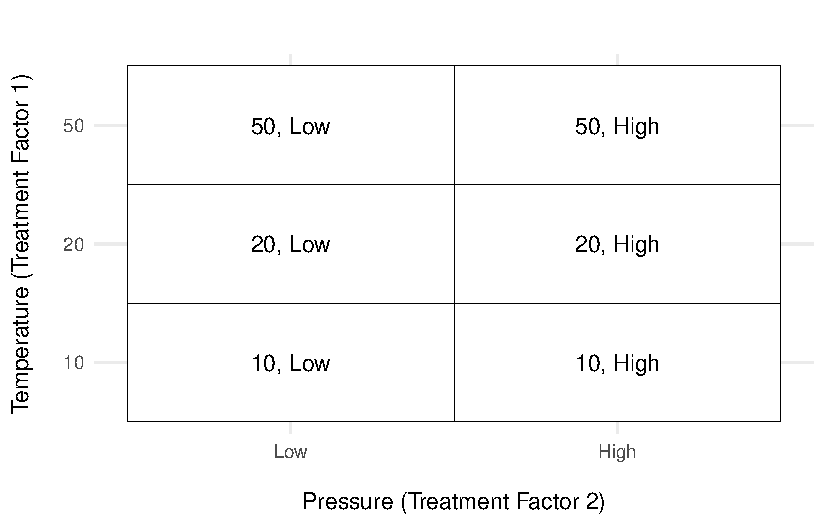
\includegraphics[keepaspectratio]{02_ExpDesign_Term_files/figure-pdf/fig-vistreat-1.pdf}}

}

\caption{\label{fig-vistreat}Visualization of how treatments are formed
as combinations of treatment levels.}

\end{figure}%

In the figure above, there are two treatment factors: Temperature (on
the y-axis) and Pressure (on the x-axis). The axis ticks represent the
levels of each treatment factor, and the blocks within the grid
represent the treatments, which are specific combinations of the levels
of Temperature and Pressure. Each treatment is labeled with the
corresponding combination of levels (e.g., `50, Low' or `10, High').

\begin{tcolorbox}[enhanced jigsaw, rightrule=.15mm, toptitle=1mm, colback=white, title={Example 1}, colframe=quarto-callout-warning-color-frame, leftrule=.75mm, opacityback=0, colbacktitle=quarto-callout-warning-color!10!white, bottomtitle=1mm, bottomrule=.15mm, arc=.35mm, titlerule=0mm, coltitle=black, left=2mm, opacitybacktitle=0.6, breakable, toprule=.15mm]

Three groups of students, 5 in each group, were receiving therapy for
severe test anxiety. Group 1 recieved 5 hours, group 2 received 10 hours
and group 3 received 15 hours. At the end of therapy each subject
completed an evaulation of test anxiety. Did the amount of therapy have
an effect on the level of test anxiety?

The three groups of studnets received the scores on the Test Anxiety
index (TAI) at the end of treatment shown in the table below.

\begin{longtable}[]{@{}ccc@{}}
\toprule\noalign{}
Group 1 & Group 2 & Group 3 \\
\midrule\noalign{}
\endhead
\bottomrule\noalign{}
\endlastfoot
48 & 55 & 51 \\
50 & 52 & 52 \\
53 & 53 & 50 \\
52 & 55 & 53 \\
50 & 53 & 50 \\
\end{longtable}

\hfill\break

\end{tcolorbox}

When faced with a text like this, it is useful to identify the treatment
factors, their levels and the treatments, as well the response. Clearly,
from the question, we are interested in the effect of therapy on test
anxiety. A statement like this can generally be read as the effect of
the treatment factor on the response. Nowhere is another treatment
factor mentioned, so we only have one in this example. What are the
levels of therapy we set? The levels are 5, 10 and 15 hours of therapy
and since we only have one factor these are also the treatments. Let's
summarise this as follows:

\begin{itemize}
\tightlist
\item
  \textbf{Response:} Test Anxiety\\
\item
  \textbf{Treatment Factor:} Therapy\\
\item
  \textbf{Treatment Levels:} 5, 10, and 15 hours of therapy\\
\item
  \textbf{Treatments:} 5, 10, and 15
\end{itemize}

\section*{\texorpdfstring{\textbf{Experimental and observational
unit}}{Experimental and observational unit}}\label{experimental-and-observational-unit}
\addcontentsline{toc}{section}{\textbf{Experimental and observational
unit}}

\markright{\textbf{Experimental and observational unit}}

The \textbf{experimental unit} is the entity (e.g.~material, object, or
individual) to which a treatment is assigned or that receives the
treatment. By contrast, the \textbf{observational unit} is the entity
from which the response is recorded. This distinction is very important
because it is the experimental units which determine how often the
treatment has been replicated and therefore the precision with which we
can measure the treatment effect. In the methods that we cover in this
course, we require that in the end there is only one `observation'
(response value) per experimental unit. If several measurements have
been taken on an experimental unit, we will combine these into one
observation, typically by taking the mean. Very often, the experimental
unit is also the observational unit.

For See Example
(\textbf{example-box?})\marginpar{\begin{footnotesize}example-box\vspace{2mm}\par\end{footnotesize}}
for more details, what are the experiemental units? To determine this,
revisit the text of Example 1 and ask yourself: what entity received the
treatments or to what were treatments applied? Most of you, will
probably answer the students and this is correct. Each student received
the respective treatment (number of hours in therapy) assigned to their
group and so there are \(5 \times 3 = 15\) experimental units.

There is an argument to be made that it is not clear whether the
students received therapy on their own or that the groups of students
received therapy together. In that case, treatments were applied to
groups of students and so there would be three experimental units. This
will usually be clear from the text, but we'll use this scenario to
illustrate some concepts as we go.

We also need to know what the observational units are. The text states
that at the end of therapy, each student completed an evaluation to
determine their level of test anxiety. So the response, test anxiety,
was measured on the student level which means students are the
observational units. In the first scenario, the students are both the
experimental units and observational units. But this would not be the
case if groups are the experimental unit.

We also require that there is only one observation per experimental
unit, the first scenario meets this requirement. For the second
scenario, we have 5 observations per group and so we would have to take
the mean of these values to end up wth one response value per group.

Let's add to the summary assuming students are the experimental units:

\begin{itemize}
\tightlist
\item
  \textbf{Experimental unit (no):} Student (15)\\
\item
  \textbf{Observational unit (no):} Student (15)
\end{itemize}

\section*{\texorpdfstring{\textbf{Homogeneity of experimental
units}}{Homogeneity of experimental units}}\label{homogeneity-of-experimental-units}
\addcontentsline{toc}{section}{\textbf{Homogeneity of experimental
units}}

\markright{\textbf{Homogeneity of experimental units}}

When the set of experimental units are as similar as possible such that
there are no distinguishable differences between them, they are said to
be \textbf{homogeneous} (a fancy word for saying they are of the same
kind). The more homogeneous the units are, the smaller the experimental
error variance (natural variation between between observations of the
same treatments) will be. It is super important to have fairly
homogeneous units because it allows us to detect differences between
treatments more easily.

\section*{\texorpdfstring{\textbf{Blocking}}{Blocking}}\label{blocking}
\addcontentsline{toc}{section}{\textbf{Blocking}}

\markright{\textbf{Blocking}}

If the experimental units are not fairly similar but are heterogeneous
(the opposite of homogeneous), we can group them into sets of similar
units. This process is called \textbf{blocking} and the groups are
considred ``blocks''. We compare the treatments within each block as if
each block is its own mini-experiment. This way we account for the
differences between blocks and can better isolate the effect of the
treatments.

\begin{tcolorbox}[enhanced jigsaw, rightrule=.15mm, toptitle=1mm, colback=white, title={Example 2.2 EDIT THIS STILL}, colframe=quarto-callout-warning-color-frame, leftrule=.75mm, opacityback=0, colbacktitle=quarto-callout-warning-color!10!white, bottomtitle=1mm, bottomrule=.15mm, arc=.35mm, titlerule=0mm, coltitle=black, left=2mm, opacitybacktitle=0.6, breakable, toprule=.15mm]

Imagine you're testing the effectiveness of two marketing strategies (A
and B) to increase sales at a chain of coffee shops. The coffee shops
are located in different neighborhoods, where factors like income levels
might influence sales. To prevent these differences from skewing the
results, you group the coffee shops into ``blocks'' based on
neighborhood income level (e.g., low, medium, high).

Within each block, you randomly assign coffee shops to either Strategy A
or Strategy B. This approach allows you to compare the strategies while
controlling for variability caused by differences in neighborhood income
levels.

Without blocking, would you be able to confidently attribute differences
in sales to the strategies alone? Likely not, as any observed
differences could be due to neighborhood-specific factors rather than
the strategies themselves.

\end{tcolorbox}

\section*{\texorpdfstring{\textbf{Replication and
pseudoreplication}}{Replication and pseudoreplication}}\label{replication-and-pseudoreplication}
\addcontentsline{toc}{section}{\textbf{Replication and
pseudoreplication}}

\markright{\textbf{Replication and pseudoreplication}}

If a treatment is applied independently to more than one experimental
unit it is said to be \textbf{replicated}. Treatments must be
replicated! Making more than one observation on the same experimental
unit is not replication, but \emph{pseudoreplication}. Pseudoreplication
is a common fallacy (REF?). The problem is that without true
replication, we don't have an estimate of uncertainty, of how
repeatable, or how variable the result is if the same treatment were to
be applied repeatedly.

In Example 1, if experimental units were the groups and we didn't take
the average of the observations per group, we would have
pseudoreplication as each student would not be an independent replicate
of a treatment - effectively, we have only applied each treatment once.
You might notice that we then only have one true replicate per treatment
group and this is problematic. To get an estimate of uncertainty, we
would have to repeat this experiment a few more times to get more than
one proper replicate.

The first scenario, however, did not have this problem and each
treatment was replicated five times. After going through all this, we
have the following summary:

\begin{itemize}
\tightlist
\item
  \textbf{Response:} Test Anxiety\\
\item
  \textbf{Treatment Factor:} Therapy\\
\item
  \textbf{Treatment Levels:} 5, 10, and 15 hours of therapy\\
\item
  \textbf{Treatments:} 5, 10, and 15\\
\item
  \textbf{Experimental unit (no):} Student (15)\\
\item
  \textbf{Observational unit (no):} Student (15)\\
\item
  \textbf{Replicates:} 5
\end{itemize}

\begin{tcolorbox}[enhanced jigsaw, rightrule=.15mm, toptitle=1mm, colback=white, title=\textcolor{quarto-callout-tip-color}{\faLightbulb}\hspace{0.5em}{Tip}, colframe=quarto-callout-tip-color-frame, leftrule=.75mm, opacityback=0, colbacktitle=quarto-callout-tip-color!10!white, bottomtitle=1mm, bottomrule=.15mm, arc=.35mm, titlerule=0mm, coltitle=black, left=2mm, opacitybacktitle=0.6, breakable, toprule=.15mm]

Creating a summary like this, is a handy exercise for any experiment you
come across, and we'll keep doing it for every experiment in this book.
As we go along, we'll also add information about the type of experiment
that was conducted.

\end{tcolorbox}

\chapter{The three R's of experimental
design}\label{the-three-rs-of-experimental-design}

\textbf{Experimental Design} is a detailed procedure for grouping, if
blocking is necessary, experimental units and for how treatments are
assigned to the experimental units. There are three fundamental
principles, known as the `three R's of experimental design' which are at
the core of a good experiment. The following section might feel a bit
repetitive, but these concepts cannot be emphasised enough.

\section{Replication}\label{replication}

Let's define it again: replication is when each treatment is applied to
several experimental units. This ensures that the variation between two
or more units receiving the same treatment can be estimated and valid
comparisons can be made between treatments. In other words, replication
allows us to separate variation due to differences between treatments
from variation within treatments. For true replication, each treatment
should be \textbf{independently} applied to several experimental units.
If this is not the case, treatment effects become confounded with other
factors.

Confounding means that is not possible to separate the effects of two
(or more) factors on the response, i.e.~it is not possible to say which
of the two factors is responsible for any changes in the response. This
is what happened in the Example 1 when groups are the experimental
units. With only one observation per experimental unit, the effect of
therapy is confounded with the experimental unit or the effect of group
on test anxiety. The reason why this is a problem is that any difference
between the treatments could be due to any differences between the
groups and not just the number of therapy hours. The same would be true
if we only had one student per group, why? Take a moment to think about
this.

Consider the first row of the data from Example 1. It looks like the
student in group 2 scored the highest, followed by group 3 and then
group 1. So does longer therapy sessions lead to higher test anxiety?
Likely not! With only one student per treatment, we are not able to say
that any differences in the response are due to the treatments. It could
be due to any differences between the individuals. Maybe the student in
group 3 tends to score higher on anxiety tests regardless of the
treatment, or perhaps the student in group 1 was unusually calm that
day. Without replication, these individual differences could mask (or
mimic) the true effects of the treatments.

By replicating the treatments across multiple students, we can average
out these individual differences and gain a clearer picture of whether
therapy duration truly impacts test anxiety. With five students per
group, we might observe that group 1 consistently scores lower than
group 3. This consistency would provide stronger evidence that the
treatments, and not just individual variation, are responsible for the
observed differences. So by replication, we can compare within treatment
variation to variation between treatments.

\begin{longtable}[]{@{}ccc@{}}
\toprule\noalign{}
Treatment 1 & Treatment 2 & Treatment 3 \\
\midrule\noalign{}
\endhead
\bottomrule\noalign{}
\endlastfoot
48 & 55 & 51 \\
50 & 52 & 52 \\
53 & 53 & 50 \\
52 & 55 & 53 \\
50 & 53 & 50 \\
\end{longtable}

\begin{tcolorbox}[enhanced jigsaw, rightrule=.15mm, toptitle=1mm, colback=white, title={Example 3.1}, colframe=quarto-callout-tip-color-frame, leftrule=.75mm, opacityback=0, colbacktitle=quarto-callout-tip-color!10!white, bottomtitle=1mm, bottomrule=.15mm, arc=.35mm, titlerule=0mm, coltitle=black, left=2mm, opacitybacktitle=0.6, breakable, toprule=.15mm]

Maybe the co2 uptake data?

\end{tcolorbox}

\section{Randomisation}\label{randomisation}

Randomisation refers to the process of randomly assigning treatments to
experimental units such that each experimental unit has equal chance of
receiving a specific treatment. Randomisation ensures that:

\begin{enumerate}
\def\labelenumi{\arabic{enumi}.}
\item
  There is no bias on the part of the experimenter, either conscious or
  unconscious, when assigning treatments to experimental units.
\item
  No experimental unit is favored to receive a particular treatment.
\item
  Possible differences between units are equally distributed amongst
  treatments. If there are clear differences between units, then
  blocking should be performed and randomisation occurs within blocks.
  We'll talk more about this in Chapter INSERT
\item
  We can assume independence between observations.
\end{enumerate}

Randomisation is not haphazard. In statistics (and here in the context
of experimental design), randomisation has a specific meaning: namely
that each experimental unit has the same chance of being allocated any
of the treatments. This can be done using random number generators such
as with software packgaes, dice or drawing number from a hat (provided
the number have been shuffled adequately and have equal chance to be
picked).

Let's have a look at randomisation in R. Suppose we have 4 treatments
(\texttt{A}, \texttt{B}, \texttt{C}, and \texttt{D}) and 32 experimental
units. There are no differences between the units, so we don't have to
block, and we can equally split the units across the treatments, which
means we have 8 units per treatment, i.e., 8 replicates. In R, we first
create a long vector of 8 \texttt{A}s, 8 \texttt{B}s, 8 \texttt{C}s, and
8 \texttt{D}s called \texttt{all.treat}. Then shuffle the vector to
obtain a randomisation using the function \texttt{sample}.

\begin{Shaded}
\begin{Highlighting}[]
\CommentTok{\# repeat the vector A, B, C, D 8 times }
\NormalTok{all.treats }\OtherTok{\textless{}{-}} \FunctionTok{rep}\NormalTok{(}\FunctionTok{c}\NormalTok{(}\StringTok{"A"}\NormalTok{,}\StringTok{"B"}\NormalTok{,}\StringTok{"C"}\NormalTok{,}\StringTok{"D"}\NormalTok{), }\AttributeTok{times =} \DecValTok{8}\NormalTok{)}

\CommentTok{\# permutation of all.treats (sample withut replacement)}
\NormalTok{rand1 }\OtherTok{\textless{}{-}} \FunctionTok{sample}\NormalTok{(all.treats)}

\CommentTok{\# example output}
\NormalTok{rand1}
\end{Highlighting}
\end{Shaded}

\begin{verbatim}
 [1] "C" "C" "A" "C" "C" "D" "A" "D" "C" "C" "D" "B" "A" "B" "C" "B" "C" "A" "D"
[20] "B" "A" "B" "A" "D" "B" "D" "A" "B" "D" "D" "B" "A"
\end{verbatim}

Experimental unit 1 recipes the first treatment that appears as the
first element in the shuffled vector, experimental unit 2 receives the
second and so on.

Notes on randomisation?

\section{Reduction of Unexplained Variation
(Blocking)}\label{reduction-of-unexplained-variation-blocking}

Unexplained variation (or experimental error variance or within
treatment variance) is largely due to inherent differences between
experimental units. The larger this unexplained variation, the more
difficult it becomes to detect treatment differences (a treatment
signal). To minimise experimental error variance we can control
extraneous factors (i.e.~keeping all else constant) and by choosing
homogeneous experimental units. Otherwise, we can \textbf{block}
experimental units to reduce the variation.

Blocking variables are nuisance factors that might affect your response
or introduce systematic variation in the response and we are typically,
not interested in these. Often, they are factors that cannot be
randomised, e.g.~biological sex of a person, time of day, location of a
warehouse etc. We control the effect of such variables on the response
by blocking for them so that we can investigate the possible effect of a
variable that we are interested in. Usually, in a \textbf{complete
block} experiment, there are as many experimental units per block as
there are treatments, so that each treatment is applied once in every
block. Treatments are randomized to the experimental units in the
blocks. We can then compare the effects of treatments on similar
experimental units, and we can estimate the variation induced in the
response due to the differences between blocks. This variation due to
blocks can then be removed from the unexplained variation.

EXAMPLE

Blocking also offers the oopurutnity to test treatments over a wider
range of conditions, e.g.~if I only use people of one age in my
experiment (say students) I cannot generalize my results to older
people. However, if i use different age blocks I will be able to tell
whether the treatments have similar effects in all age groups or not.

Lastly, if blocking is not feasible, randomization will ensure that at
least treatments and nuisance factors are not confounded.

\begin{quote}
``Block what you can, randomize what you cannot.''

--- Box, Hunter \& Hunter (1978)
\end{quote}

\chapter{Designing an Experiment}\label{designing-an-experiment}

When planning an experiment we need to decide on:

\begin{itemize}
\tightlist
\item
  treatment factors and their levels
\item
  the response
\item
  experimental material / units
\item
  blocking factors
\item
  number of replicates
\end{itemize}

Some of these will be determined by the research question and how
experimental units are assigned to treatments are determined by the
design. The design that will be chosen for a particular experiment
depends on the \textbf{treatment structure} (determined by the research
question) and the \textbf{blocking structure} (determined by the
available experimental units).

Here are two ways the treatments can be structured:

\begin{enumerate}
\def\labelenumi{\arabic{enumi}.}
\tightlist
\item
  \textbf{Single factor}: the treatments are the levels of a single
  treatment factor.
\item
  \textbf{Factorial}: when more than one factor are of interest, then
  the experiment is said to be a factorial experiment. The treatments
  are constructed by crossing the treatment factors like we did in
  Figure~\ref{fig-vistreat} such that the treatments are all possible
  combinations of the treatment levels. For example, if factor A has
  \(a\) levels and factor B has \(b\) levels, there are \(a \times b\)
  treatments. Such an experiment would then be called an \(a \times b\)
  factorial experiment.
\end{enumerate}

The blocking structure is determined the set of experimental units
chosen or available for the experiment.are there any
structures/differences that need to be blocked? Do I want to include
experimental units of different types to make the results more general?
How many experimental units are available in each block? For the
simplest design in this course, the number of experimental units in each
block corresponds to the number of treatments. This is called a complete
block experiment. There are several other blocking structures, such as
incomplete blocks and blocks with missing values, all with specific
analysis which we will not cover here.

In this course, we cover two basic designs: Completely Randomized
Designs (CRD) and Randomized Block Designs (RBD). For both designs, the
treatment structure can be single or factorial. Where they differ is in
terms of the experimental units and how randomization occurs.

\textbf{\emph{Completely Randomized Designs (CRD)}}

When all experimental units are fairly homogeneous, a CRD is used.
Treatments are randomized to all experimental units.

\textbf{\emph{Randomized Block Design}}

This design is used when all experimental units are not homogeneous or
blocking is required to control a nuisance factor. The treatments are
randomized to the units within blocks.

\part{Single Factor Completely Randomised Designs}

\chapter{Introduction}\label{introduction}

Completely Randomized Designs (CRDs) are the simplest experimental
designs. They are used when experimental units are uniform enough. We
expect them to react simirlary to a given treatment; we have no reason
to suspect that a group of experimental units might react differently to
the treatments. We also don't expect any effects (besides possibly a
treatment effect) to cause any systematic changes in the response. In
other words, we don't have to block for nuisance factors.

Remember experimental design is the procedure for how experimental units
are grouped and treatments are applied. We have already said that there
are no blocks in CRDs. So randomisation occurs without restriction and
to all experimental units. More generally, the \(a\) treatments are
randomly assigned to \(r\) experimental units, such that each
experimental unit is equally likely to receive any of the treatments.
This means that there are \(N = r \times a\) experimentnal units in
total. We only consider designs that are \emph{balanced} meaning that
there an equal number of experimental units per treatment, i.e.~a
treatment is applied to \(r\) units.

\section{Example: The effect of social media multitasking on classroom
performance.}\label{example-the-effect-of-social-media-multitasking-on-classroom-performance.}

Can we really multitask? I remember as a student I thought I could
multitask in lectures, while studying or driving and listening to a
podcast. It felt like I was paying attention but in hindsight I can't
remember those podcasts well, I know I had to revisit lectures and
restart studying sessions. This extends beyond student life, where in
the average workspace, tasks are interspersed with social media or email
checks and notifcations (). I think most of us are almost always a
little bit tempted by our cellphones when we study or work.

So, if we live in an age of perceived multitasking and getting
distracted by our phones and devices, what are the efffects of social
media multitasking on our academic performance?

\begin{tcolorbox}[enhanced jigsaw, rightrule=.15mm, toptitle=1mm, colback=white, title={Example 5.1}, colframe=quarto-callout-warning-color-frame, leftrule=.75mm, opacityback=0, colbacktitle=quarto-callout-warning-color!10!white, bottomtitle=1mm, bottomrule=.15mm, arc=.35mm, titlerule=0mm, coltitle=black, left=2mm, opacitybacktitle=0.6, breakable, toprule=.15mm]

Two researchers from Turkey, Demirbilek and Talan
(2018)\marginpar{\begin{footnotesize}
\begin{CSLReferences}{2}{0}
\bibitem[\citeproctext]{ref-multitask2018}
Demirbilek, Muhammet, and Tarik Talan. 2018. {``The Effect of Social
Media Multitasking on Classroom Performance.''} \emph{Active Learning in
Higher Education} 19 (2): 117--29.
\end{CSLReferences}
\vspace{2mm}\par\end{footnotesize}},
conducted a study to investigate this question. Specifically, they
examined the impact of social media multitasking during live lectures on
students' academic performance.

A total of 120 undergraduate students were randomly assigned to one of
three groups:

\begin{enumerate}
\def\labelenumi{\arabic{enumi}.}
\tightlist
\item
  \textbf{Control Group:} Students used traditional pen-and-paper
  note-taking.
\item
  \textbf{Experimental Group 1 (Exp 1):} Students engaged in SMS texting
  during the lecture.
\item
  \textbf{Experimental Group 2 (Exp 2):} Students used Facebook during
  the lecture.
\end{enumerate}

Over a three-week period, participants attended lectures on Microsoft
Excel. Pre-tests and post-tests were administered to measure learning
outcomes.

\end{tcolorbox}

\textbf{The analysis of experimental data is determined by the design.}
The design dictates the terms that we will include in our statistical
model and so it is crucial to be able to identify the design and
blocking and treatment factors. It is also important to check that
randomisation has been done correctly and determine the number of
replicates used. In the previous chapter we started doing this by
creating a summary of the design and we do the same here. From the
description of the study, it is clear that:

\begin{itemize}
\tightlist
\item
  \textbf{Response Variable:} Academic performance, as measured by test
  scores.
\item
  \textbf{Treatment Factor:} Level of social media multitasking.
\item
  \textbf{Treatment Levels (Groups):} Control, Exp 1, and Exp 2.
\end{itemize}

Students were randomly assigned to one of the three groups, and
performance was measured for each individual. Although this may seem
obvious, they only took one measurement per student, so we don't have to
worry about pseudoreplication. This setup indicates that the students
are both the experimental units and the observational units in this
study. With a total of 120 experimental units and three treatments, the
experiment has 40 replicates. Since only one treatment factor was
investigated, and no blocking was performed, this is classified as a
\textbf{single-factor Completely Randomized Design (CRD).} Here is the
study breakdown:

\begin{itemize}
\tightlist
\item
  \textbf{Response Variable:} Academic Performance\\
\item
  \textbf{Treatment Factor:} Level of Social Media Multitasking\\
\item
  \textbf{Treatment Levels:} Control, Experimental 1 (SMS), Experimental
  2 (Facebook)\\
\item
  \textbf{Treatments:} Control, SMS multitasking, Facebook
  multitasking\\
\item
  \textbf{Experimental Unit:} Student (120)\\
\item
  \textbf{Observational Unit:} Student (120)\\
\item
  \textbf{Replicates:} 40 students per group\\
\item
  \textbf{Design Type:} Single-Factor Completely Randomized Design (CRD)
\end{itemize}

Before we continue, now is the time to note that we won't be using the
real data collected in this experiment. It wasn't available but I have
simulated data to match their results. I've also made some other
modifications such as the original study included 122 students but to
ensure a balanced design I include only 120.

\section{Exploratory data analysis}\label{exploratory-data-analysis}

Before we start any analyses, two things need to be done. First, we
start by exploring our data to get familar with the format and to get a
feel for any patterns. In R, we read in the data set and then peform a
few fommands to check the dataset:

\begin{Shaded}
\begin{Highlighting}[]
\NormalTok{multitask }\OtherTok{\textless{}{-}} \FunctionTok{read.csv}\NormalTok{(}\StringTok{"multitask\_performance.csv"}\NormalTok{)}
\FunctionTok{nrow}\NormalTok{(multitask) }\CommentTok{\# check number of rows}
\end{Highlighting}
\end{Shaded}

\begin{verbatim}
[1] 120
\end{verbatim}

\begin{Shaded}
\begin{Highlighting}[]
\FunctionTok{head}\NormalTok{(multitask) }\CommentTok{\# check first 5 rows }
\end{Highlighting}
\end{Shaded}

\begin{verbatim}
    Group Posttest
1    Exp1 86.39427
2    Exp1 64.19996
3    Exp2 52.75394
4 Control 67.81147
5    Exp1 52.39911
6    Exp1 56.58150
\end{verbatim}

\begin{Shaded}
\begin{Highlighting}[]
\FunctionTok{tail}\NormalTok{(multitask) }\CommentTok{\# check last 5 rows }
\end{Highlighting}
\end{Shaded}

\begin{verbatim}
      Group Posttest
115 Control 77.94344
116 Control 63.58444
117    Exp1 55.17758
118    Exp2 67.16150
119    Exp2 32.58373
120    Exp2 49.58119
\end{verbatim}

\begin{Shaded}
\begin{Highlighting}[]
\FunctionTok{summary}\NormalTok{(multitask)}
\end{Highlighting}
\end{Shaded}

\begin{verbatim}
    Group              Posttest    
 Length:120         Min.   :23.38  
 Class :character   1st Qu.:52.67  
 Mode  :character   Median :65.01  
                    Mean   :63.59  
                    3rd Qu.:76.32  
                    Max.   :98.78  
\end{verbatim}

The dataset consits of 120 rows (each row representing a student) and
two columns (\texttt{Group} and \texttt{Posttest}). The first column,
\texttt{Groups}, contains the treatment the student was assigned and the
\texttt{Posttest} column contains the response measure. Using the
functions \texttt{head} and \texttt{tail}, we can look at the first and
last 5 rows and the function \texttt{summary} provies us with a
descrption of each column. We do this to check that R has read in our
data correctly (you can view the whole data set by running
\texttt{view(multitask)} as well). The summary tells us that the
\texttt{Group} column is of the class ``character''. For our analysis,
we want it to be read as a factor:

\begin{Shaded}
\begin{Highlighting}[]
\NormalTok{multitask}\SpecialCharTok{$}\NormalTok{Group }\OtherTok{\textless{}{-}} \FunctionTok{as.factor}\NormalTok{(multitask}\SpecialCharTok{$}\NormalTok{Group)}
\FunctionTok{summary}\NormalTok{(multitask)}
\end{Highlighting}
\end{Shaded}

\begin{verbatim}
     Group       Posttest    
 Control:40   Min.   :23.38  
 Exp1   :40   1st Qu.:52.67  
 Exp2   :40   Median :65.01  
              Mean   :63.59  
              3rd Qu.:76.32  
              Max.   :98.78  
\end{verbatim}

Now, we can see that there are 40 replicates per treatment group,
confirming that the experiment was balanced. I have assumed that based
on the resuts shown that the \texttt{Posttest} scores were stored as
percentages and using the sumamry we can quickly checked whether there
are any observations that are not on the appropriate scale. Looks good
so far!

\section{Model checking}\label{model-checking}

Demirbilek and Talan
(2018)\marginpar{\begin{footnotesize}
\begin{CSLReferences}{2}{0}
\bibitem[\citeproctext]{ref-multitask2018}
Demirbilek, Muhammet, and Tarik Talan. 2018. {``The Effect of Social
Media Multitasking on Classroom Performance.''} \emph{Active Learning in
Higher Education} 19 (2): 117--29.
\end{CSLReferences}
\vspace{2mm}\par\end{footnotesize}}
had several research questions, but here we only consider the following:
Are there any signficant differences in mean academic performance
between the three groups?

You might think that we could perform three t-tests (Control vs Exp 1,
Control vs Exp 3, Exp 1 vs Exp 2). We could, but the problem with this
approach is what we call mutliple testing. When conducting many tests,
there is an increased risk of making a Type 1 Error (rejecting the null
hypothesis when it is in fact true) \sidenote{\footnotesize Can't remember what a
  \(t\)-test is and/or need a refresher on hypothesis testing? Have a
  look this video on t-tests and document for a brief reminder.
  \textbf{Also, a quick (and cool) sidenote:} This study by Chen et al.
  (2024) used a Completely Randomized Design (CRD), randomly assigning
  undergraduate students to playback speed groups (1x, 1.5x, 2x, and
  2.5x) to measure the effect on comprehension of recorded lectures.
  Using ANOVA they found that comprehension was preserved up to 2x
  speed. I personally like to increase the playback speed to 1.5px if I
  just need to revise something
  quickly.\linebreak\linebreak
\begin{CSLReferences}{2}{0}
\bibitem[\citeproctext]{ref-chen2024effect}
Chen, Ashley, Suchita E Kumar, Rhea Varkhedi, and Dillon H Murphy. 2024.
{``The Effect of Playback Speed and Distractions on the Comprehension of
Audio and Audio-Visual Materials.''} \emph{Educational Psychology
Review} 36 (3): 79.
\end{CSLReferences}
\linebreak}.

When we have more than two groups, we can use a one-way analysis of
variance (ANOVA) which can be seen as an extention of \(t\)-test and is
called one-way because there is a single factor being considered. For
both of these statistical approaches the data should meet certain
distributional assumptions:

\begin{enumerate}
\def\labelenumi{\arabic{enumi}.}
\tightlist
\item
  There are no outliers.
\item
  All groups have equal population variances.
\item
  The errors are normally distributed.
\item
  The errors are independent.
\end{enumerate}

\subsection*{Outliers}\label{outliers}
\addcontentsline{toc}{subsection}{Outliers}

Outliers are unusual observations (response values) that deviate
substantially from the remaining data points. They can have a large
influence on the estimates of our model. Think of statistics such as
means and variances, outlying observations will shift the mean towards
them and distort the variance of the data.

Sometimes outliers are artefacts of data recording/entering issues, such
as a missing decimal points or incorrect scaling (called error
outliers). These types of outliers can be corrected and the analysis can
be done as usual. If, however, there are freak observations that are not
clearly due to anything like data inputting, then they are likely
unusual responses and should not be discarded (interesting outliers).
There are many ways of identifying and dealing with outliers
((\textbf{outlier?})\marginpar{\begin{footnotesize}outlier\vspace{2mm}\par\end{footnotesize}}
found 29 different ways). Here, it is recommended that the analyses
should then be run with and without the outliers to see whether the
conclusion depends on their inclusion. When dealing with outliers, it is
best to be transparent and clear about how they were handled. Simply
removing outliers with no explanation is questionable research practice.

A good way to check for outliers, is to inspect the data visually with a
boxplot of your data grouped by treatment.

\begin{Shaded}
\begin{Highlighting}[]
\FunctionTok{boxplot}\NormalTok{(Posttest }\SpecialCharTok{\textasciitilde{}}\NormalTok{ Group, }\AttributeTok{data =}\NormalTok{ multitask, }\AttributeTok{col =} \FunctionTok{c}\NormalTok{(}\StringTok{"skyblue"}\NormalTok{, }\StringTok{"lightgreen"}\NormalTok{, }\StringTok{"pink"}\NormalTok{), }
        \AttributeTok{main =} \StringTok{"Posttest Scores by Group"}\NormalTok{, }
        \AttributeTok{xlab =} \StringTok{"Group"}\NormalTok{, }
        \AttributeTok{ylab =} \StringTok{"Posttest Scores"}\NormalTok{)}

\FunctionTok{stripchart}\NormalTok{(Posttest}\SpecialCharTok{\textasciitilde{}}\NormalTok{Group, }\AttributeTok{data =}\NormalTok{ multitask, }\AttributeTok{vertical =} \ConstantTok{TRUE}\NormalTok{, }\AttributeTok{add =} \ConstantTok{TRUE}\NormalTok{, }\AttributeTok{method =} \StringTok{"jitter"}\NormalTok{)}
\end{Highlighting}
\end{Shaded}

\pandocbounded{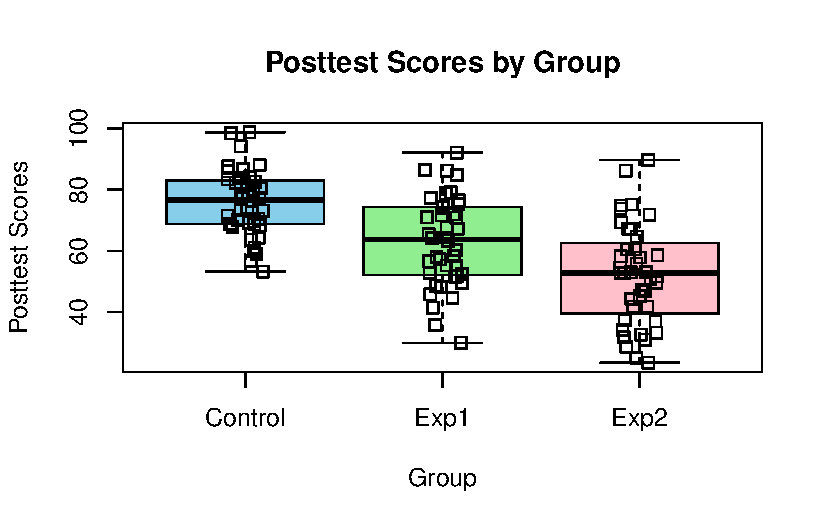
\includegraphics[keepaspectratio]{05_CRD_Intro_files/figure-pdf/plot-1.pdf}}

The first line of code plots the boxplot and by inputting
\texttt{Posttest\textasciitilde{}Groups} as the first argument we are
say plot the values of \texttt{Posttest} by \texttt{Groups}. There are
extra graphical parameters specfied to make the plot look a bit nicer.
Then the function \texttt{stripchart} is used to overlay the data
points. Based on these plots, there aren't any obvious outlying
observations.

\subsection*{Equal population
variances}\label{equal-population-variances}
\addcontentsline{toc}{subsection}{Equal population variances}

Since we only have sample data, we would not expect that the variance in
each treatment are the same, so just because they are different does not
mean the population variances are different. We expect them to differ a
bit due to chance simply because we are sampling from a population and
everytime we take a sample, the dataset will be different. The sample
variances need to be similar enough so that our assumption of qual
population variances is reasonable. To check this assumption, we can
inspect the boxplots again and their respective heights. More
specifically, we look at the interquartile ranges. From looking at the
plot, the IQRs do not vary widely. If you prefer to look at the actual
values, we can use R to obtain them:

\begin{Shaded}
\begin{Highlighting}[]
\FunctionTok{sort}\NormalTok{(}\FunctionTok{tapply}\NormalTok{(multitask}\SpecialCharTok{$}\NormalTok{Posttest,multitask}\SpecialCharTok{$}\NormalTok{Group,IQR))}
\end{Highlighting}
\end{Shaded}

\begin{verbatim}
 Control     Exp2     Exp1 
14.01068 20.94529 21.97001 
\end{verbatim}

Another measure of variability we can look at, are the standard
deviations (sd's). With the same line of code but just replacing the
function we want to apply, we obtain the sd's of each group:

\begin{Shaded}
\begin{Highlighting}[]
\FunctionTok{sort}\NormalTok{(}\FunctionTok{tapply}\NormalTok{(multitask}\SpecialCharTok{$}\NormalTok{Posttest,multitask}\SpecialCharTok{$}\NormalTok{Group,sd))}
\end{Highlighting}
\end{Shaded}

\begin{verbatim}
 Control     Exp1     Exp2 
10.82887 14.60601 16.42678 
\end{verbatim}

The rule of thumb is to use the ratio of the smallest to largest
standard deviation and check whether it is smaller than five. In our
case, the smallest sd (of the Control group) is about 1.5 times smaller
than the largest sd (of the Exp 2 group)n .

\subsection*{Normally distributed
errors}\label{normally-distributed-errors}
\addcontentsline{toc}{subsection}{Normally distributed errors}

\subsection*{Independent erros}\label{independent-erros}
\addcontentsline{toc}{subsection}{Independent erros}

TIPS:

\begin{itemize}
\tightlist
\item
  increase focus, improve studying
\end{itemize}

\chapter{A Simple Model for a CRD}\label{a-simple-model-for-a-crd}

\chapter{Analysis of Variance}\label{analysis-of-variance}

Although, I like the following description:

\begin{quote}
``Analysis of variance is better defined as a method of dividing
(analysing) a total variance into at least two components\ldots Using a
liberal definition of variances, analysis of variance can be said to
consist of estimating variances, and possibly of testing hypotheses
about them.''

--- Paul Seeger (1966)
\end{quote}

\chapter{Contrasts}\label{contrasts}

\part{Randomised Block Designs}

\part{Factorial Experiments}

\bookmarksetup{startatroot}

\chapter*{Glossary}\label{glossary}
\addcontentsline{toc}{chapter}{Glossary}

\markboth{Glossary}{Glossary}

\begin{description}
\item[\phantomsection\label{glossary-experimental-design}{Experimental
Design}]
A systematic method to plan experiments in a way that ensures valid and
unbiased results.
\item[\phantomsection\label{glossary-anova-analysis-of-variance}{ANOVA
(Analysis of Variance)}]
A statistical method used to compare the means of three or more groups
to determine if at least one differs significantly.
\item[\phantomsection\label{glossary-replication}{Replication}]
When treatments are applied to more than one experimental unit. The
number of experimental units per treatment is the number of replicates
an experiment has.
\item[\phantomsection\label{glossary-randomization}{Randomization}]
A process of randomly assigning subjects or experimental units to
treatments.
\item[\phantomsection\label{glossary-blocking}{Blocking}]
A technique to account for variability by grouping similar experimental
units.
\item[\phantomsection\label{glossary-factor}{Treatment Factor}]
An independent variable in an experiment.
\item[\phantomsection\label{glossary-level}{Treatment Level}]
The specific values or categories of a factor.
\end{description}

{[}Treatments{]}





\end{document}
